
% Options for packages loaded elsewhere
\PassOptionsToPackage{unicode}{hyperref}
\PassOptionsToPackage{hyphens}{url}
\PassOptionsToPackage{dvipsnames,svgnames,x11names}{xcolor}
\documentclass[10pt]{article}
\usepackage{xcolor}
\usepackage{amsmath,amssymb}
\setcounter{secnumdepth}{3}
\usepackage{iftex}
\ifPDFTeX
  \usepackage[T1]{fontenc}
  \usepackage[utf8]{inputenc}
  \usepackage{textcomp} % provide euro and other symbols
\else % if luatex or xetex
  \usepackage{unicode-math} % this also loads fontspec
  \defaultfontfeatures{Scale=MatchLowercase}
  \defaultfontfeatures[\rmfamily]{Ligatures=TeX,Scale=1}
\fi
\usepackage{lmodern}
\ifPDFTeX\else
  % xetex/luatex font selection
\fi
% Use upquote if available, for straight quotes in verbatim environments
\IfFileExists{upquote.sty}{\usepackage{upquote}}{}
\IfFileExists{microtype.sty}{% use microtype if available
  \usepackage[]{microtype}
  \UseMicrotypeSet[protrusion]{basicmath} % disable protrusion for tt fonts
}{}
\makeatletter
\@ifundefined{KOMAClassName}{% if non-KOMA class
  \IfFileExists{parskip.sty}{%
    \usepackage{parskip}
  }{% else
    \setlength{\parindent}{0pt}
    \setlength{\parskip}{6pt plus 2pt minus 1pt}}
}{% if KOMA class
  \KOMAoptions{parskip=half}}
\makeatother
\usepackage{longtable,booktabs,array}
\usepackage{caption}
\captionsetup[table]{skip=6pt}
\newcounter{none} % for unnumbered tables
\usepackage{calc} % for calculating minipage widths
% Correct order of tables after \paragraph or \subparagraph
\usepackage{etoolbox}
\makeatletter
\patchcmd\longtable{\par}{\if@noskipsec\mbox{}\fi\par}{}{}
\makeatother
% Allow footnotes in longtable head/foot
\IfFileExists{footnotehyper.sty}{\usepackage{footnotehyper}}{\usepackage{footnote}}
\makesavenoteenv{longtable}
\usepackage{graphicx}
\makeatletter
\newsavebox\pandoc@box
\newcommand*\pandocbounded[1]{% scales image to fit in text height/width
  \sbox\pandoc@box{#1}%
  \Gscale@div\@tempa{\textheight}{\dimexpr\ht\pandoc@box+\dp\pandoc@box\relax}%
  \Gscale@div\@tempb{\linewidth}{\wd\pandoc@box}%
  \ifdim\@tempb\p@<\@tempa\p@\let\@tempa\@tempb\fi% select the smaller of both
  \ifdim\@tempa\p@<\p@\scalebox{\@tempa}{\usebox\pandoc@box}%
  \else\usebox{\pandoc@box}%
  \fi%
}
% Set default figure placement to htbp
\def\fps@figure{htbp}
\makeatother
\ifLuaTeX
\usepackage[bidi=basic,shorthands=off]{babel}
\else
\usepackage[bidi=default,shorthands=off]{babel}
\fi
\ifLuaTeX
  \usepackage{selnolig} % disable illegal ligatures
\fi
\setlength{\emergencystretch}{3em} % prevent overfull lines
\providecommand{\tightlist}{%
  \setlength{\itemsep}{0pt}\setlength{\parskip}{0pt}}
\usepackage[]{natbib}
\bibliographystyle{tmlr}
\usepackage{tmlr}
\renewcommand{\arraystretch}{1.35}
\setlength{\extrarowheight}{3pt}
% Table rows in a survey carry paragraphs, not single words, and pandoc's
% longtables set them solid. Both knobs are needed: \arraystretch scales the
% row strut, \extrarowheight lifts the text off the rule above it.
\renewcommand{\arraystretch}{1.35}
\setlength{\extrarowheight}{3pt}
\usepackage{bookmark}
\IfFileExists{xurl.sty}{\usepackage{xurl}}{} % add URL line breaks if available
\urlstyle{same}
% fallback for those not using the hyperref driver hyperxmp:
\makeatletter
\@ifundefined{xmpquote}{\newcommand{\xmpquote}[1]{#1}}{}
\makeatother
\hypersetup{
  pdftitle={Spoken-Digit Recognition Without Training: Geometry{,} Coupling{,} and Drive Effects in Frozen Oscillator Fields},
  pdflang={en-GB},
  pdfkeywords={\xmpquote{coupled oscillators}, \xmpquote{reservoir
computing}, \xmpquote{speech recognition}, \xmpquote{Kuramoto
model}, \xmpquote{Stuart-Landau}, \xmpquote{lattice geometry}},
  colorlinks=true,
  linkcolor={RoyalBlue},
  filecolor={Maroon},
  citecolor={RoyalBlue},
  urlcolor={RoyalBlue},
  pdfcreator={LaTeX via pandoc}}
% Float placement. LaTeX's defaults reserve most of a page for text, so a
% figure taller than about a third of the block gets deferred, often past the
% section that introduces it: the physics timeline was landing inside the
% neuroscience subsection. These let a float take more of the page it belongs
% on, which keeps figures with the prose that references them.
\renewcommand{\topfraction}{0.92}
\renewcommand{\bottomfraction}{0.85}
\renewcommand{\textfraction}{0.06}
\renewcommand{\floatpagefraction}{0.72}
\setcounter{topnumber}{3}
\setcounter{bottomnumber}{2}
\setcounter{totalnumber}{4}
% Pandoc emits figures with the default [tbp], so a float can only ever move
% forward to the top of a later page. `!htbp` adds "here" and tells LaTeX to
% ignore the size fractions when deciding, which is what actually keeps a tall
% figure in the subsection that introduces it rather than a page or two later.
\makeatletter
\renewcommand{\fps@figure}{!htbp}
\renewcommand{\fps@table}{!htbp}
\makeatother
% A float may still drift past the heading of the subsection that introduces it,
% which reads as though it belongs to the next one: the physics timeline was
% landing under "Within neuroscience". Flushing pending floats at every
% subsection boundary keeps each figure inside the subsection that cites it.
% placeins would do this, but it is not in a BasicTeX installation, and the
% mechanism is short: if any float is still waiting when a subsection begins,
% flush it first. \@deferlist holds exactly those floats, so the page break
% only fires when one is actually pending.
\makeatletter
\newcommand{\tmlr@floatbarrier}{\par\vspace{\z@}%
  \ifx\@deferlist\@empty\else\clearpage\fi}
\let\tmlr@subsection\subsection
\renewcommand{\subsection}{\tmlr@floatbarrier\tmlr@subsection}
\let\tmlr@subsubsection\subsubsection
\renewcommand{\subsubsection}{\tmlr@floatbarrier\tmlr@subsubsection}
\makeatother

\hypersetup{pdfauthor={}}

\def\month{MM}
\def\year{YYYY}
\def\openreview{\url{https://openreview.net/forum?id=XXXX}}

\title{Spoken-Digit Recognition Without Training: Geometry, Coupling,
and Drive Effects in Frozen Oscillator Fields}

\author{\name }
\date{}

\begin{document}
\maketitle
\begin{abstract}
Recent work has revived coupled-oscillator networks as a computational
substrate, with several lines reporting that oscillator dynamics carry
useful task structure even without training. We test that proposition
for speech at a deliberately small, fully controlled scale. We freeze
every physics parameter of a 1,024-oscillator field (\textasciitilde2k
parameters) and measure spoken-digit recognition (AudioMNIST, speaker-
disjoint) across a full factorial of six coupling laws, six lattice
geometries, three natural-frequency structures, pinning, spectral clamp,
and three drive pathways, at three noise and gain conditions, against
five trained conventional baselines at exact parameter parity, a
no-dynamics linear floor, and published oscillator-reservoir anchors.
Untrained fields sit at a statics plateau roughly three points above a
linear ridge on band statistics at every condition tested, above every
trained conventional baseline at the same parameter budget, yet never
far above what their own input representation supports linearly, and no
design axis we varied moved that margin, with one exception:
phase-referenced drive is not merely worse untrained but unreadable. On
an order-discrimination task built so that order-free readouts provably
cannot answer it, the same frozen fields read temporal order at 0.97 to
1.00, and a severed-coupling control attributes that memory
predominantly to per-oscillator phase integration.
\end{abstract}

\section{Introduction}\label{introduction}

Coupled oscillators are having a revival as a machine-learning
substrate. Hardware reservoirs classify spoken digits with a handful of
spintronic oscillators \citep{torrejon2017}; oscillator-inspired
recurrent networks post competitive accuracy on speech-adjacent
benchmarks \citep{rusch2021}; trained Kuramoto dynamics generate images
\citep{unconv-ai2026} and function as computational primitives for
vision and reasoning \citep{miyato2025}. Much of this literature
carries, implicitly or explicitly, a reservoir premise: that oscillator
physics \emph{by itself}, before any training, transduces signals into
computationally useful structure.

This paper tests that premise for speech, under controls, at small
scale. Our overarching hypothesis, stated so it can fail:
\textbf{untrained oscillator fields possess reservoir properties useful
for speech recognition.} We commit to both outcomes. If the hypothesis
holds, the experiments say which geometries and coupling laws carry the
effect and why the data suggests so. If it does not, the experiments say
what bounds it, which design limitations could mask a real effect
(readout capacity, readout data size, field size, frontend
conditioning), each with a measured control or a named future test, and
what would refute or rescue the claim.

We evaluate spoken digits 0--9 (AudioMNIST \citep{becker2024},
speaker-disjoint split), the standard task of the oscillator-reservoir
literature, which makes our numbers placeable against published anchors
without head-to-head claims. The design principles throughout:

\begin{itemize}
\tightlist
\item
  \textbf{One change at a time.} Every comparison differs from its twin
  by exactly one factor; every scaffold is shared verbatim across arms.
\item
  \textbf{Pre-registration.} Decision bars were recorded before each
  launch; verdicts are scored per the criteria as written. Two
  registered predictions were refuted by their own tests; both
  refutations are reported.
\item
  \textbf{Attribution by construction.} The only fitted object anywhere
  in the primary protocol is a closed-form linear probe; a no-dynamics
  floor (the identical probe on the raw frontend features) decomposes
  every accuracy into what the representation carries plus what the
  dynamics add.
\item
  \textbf{The full matrix is the result.} Dead regions are reported as
  data; no runs were pruned.
\end{itemize}

Contributions:

\begin{enumerate}
\def\labelenumi{\arabic{enumi}.}
\tightlist
\item
  The first controlled comparison of lattice geometry in an oscillator
  network (six shapes at identical parameter budget and coupling
  stencil); measured effects fell well below the pre-registered
  threshold at this scale.
\item
  A three-rung transduction ladder (envelope, phase-referenced, carrier)
  that isolates \emph{how audio enters the field} as an experimental
  factor, with a drive-unit calibration protocol and an
  integrator-validity bound that any cross-frontend comparison needs.
\item
  A measured account of the phase-referenced collapse: untrained fields
  cannot read Adler-form drive at any gain, while the same pathway
  trains healthily, with the locking-range analysis that explains both
  regimes of the failure.
\item
  A readout-sufficiency control showing the linear probe is
  near-complete for these features, and quantifying the one regime where
  it is not.
\item
  Direct evidence against tonotopic frequency design under every drive
  form tested, including the case where the designed rows demonstrably
  lock to their carriers.
\item
  A suggested, evidence-bounded non-monotone relation between field
  coherence and readability.
\item
  A statics-proof order-discrimination task, floored at chance by
  construction, on which untrained oscillator state reads temporal order
  at 0.97--1.00, with a severed-coupling control that attributes the
  memory predominantly to per-oscillator integration.
\end{enumerate}

\section{Background: the physics under
test}\label{background-the-physics-under-test}

\subsection{Coupling laws}\label{coupling-laws}

All six families share the update \ensuremath{\dot{\theta}_{i}} =
\ensuremath{\omega_{i}} + coupling\ensuremath{_{i}}(\ensuremath{\theta};
K) + drive\ensuremath{_{i}} \ensuremath{-} \ensuremath{\lambda\cdot}sin
\ensuremath{\theta_{i}}, where K is a per-channel spatial coupling
kernel applied convolutionally over the lattice, \ensuremath{\omega} the
natural frequencies, \ensuremath{\lambda} a pinning toward rest, and the
drive enters per the pathway (§4.3). The families differ only in the
coupling term, a controlled deviation series from the Kuramoto base:

{\def\LTcaptype{none} % do not increment counter
\begin{longtable}[]{@{}
  >{\raggedright\arraybackslash}p{(\linewidth - 6\tabcolsep) * \real{0.2500}}
  >{\raggedright\arraybackslash}p{(\linewidth - 6\tabcolsep) * \real{0.2500}}
  >{\raggedright\arraybackslash}p{(\linewidth - 6\tabcolsep) * \real{0.2500}}
  >{\raggedright\arraybackslash}p{(\linewidth - 6\tabcolsep) * \real{0.2500}}@{}}
\toprule\noalign{}
\begin{minipage}[b]{\linewidth}\raggedright
family
\end{minipage} & \begin{minipage}[b]{\linewidth}\raggedright
coupling (essence)
\end{minipage} & \begin{minipage}[b]{\linewidth}\raggedright
primary source
\end{minipage} & \begin{minipage}[b]{\linewidth}\raggedright
why it is in the matrix
\end{minipage} \\
\midrule\noalign{}
\endhead
\bottomrule\noalign{}
\endlastfoot
kuramoto & \ensuremath{\Sigma_{j}} K\ensuremath{_{ij}}
sin(\ensuremath{\theta_{j}-\theta_{i}}) &
\citep{winfree1967, kuramoto1975} & the minimal, exactly analyzed
synchronization law; every other family is a controlled deviation from
it \\
\cmidrule{1-4}sakaguchi & sin(\ensuremath{\theta_{j}-\theta_{i}-\alpha})
& \citep{sakaguchi1986} & frustration shifts the synchronization
transition and admits travelling/partially coherent regimes
\citep{abrams2004} \\
\cmidrule{1-4}harmonic2 & + \ensuremath{\beta\cdot}sin
2(\ensuremath{\theta_{j}-\theta_{i}}) & \citep{daido1992, hansel1993} &
higher harmonics create multi-cluster attractors; cluster states as
candidate feature diversity \\
\cmidrule{1-4}winfree & sensitivity \ensuremath{\times} influence
product & \citep{winfree1967}; ML neighbor \citep{dai2026} & the
ancestral population model, a genuinely different signal pathway \\
\cmidrule{1-4}stuart--landau (sl) & complex ż =
(\ensuremath{\mu}+i\ensuremath{\omega})z \ensuremath{-}
\textbar z\textbar{}\ensuremath{^{2}}z + coupling &
\citep{stuart1960, aranson2002} & adds the amplitude channel: extra
state per oscillator \\
\cmidrule{1-4}sl-fixedamp & SL coupling, amplitude clamped & this work &
isolates coupling-form credit from amplitude-channel credit \\
\end{longtable}
}

Untrained sakaguchi/harmonic2 runs run at canonical nonzero parameters
(\ensuremath{\alpha} = \ensuremath{\pi}/4, \ensuremath{\beta} = 0.5)
because their zero values are exactly the Kuramoto reference (zero is
the correct \emph{training} initialization, where the deviation is
learned; it is not a distinct untrained physics). Both canonical values
are sensitivity-tested in §5.5.

\subsection{Lattice geometries}\label{lattice-geometries}

Six shapes share the identical local coupling stencil and parameter
budget; only the wrap rule at the lattice edge differs: sheet (both axes
open), cylinder (one periodic axis), torus (both periodic), helix (a 1-D
circulant winding with octave-per-turn tonotopy), cube (a 3-torus), and
a latitude--longitude sphere lattice. Why shape could plausibly matter
for audio, each hypothesis falsifiable in the matrix: (i) \emph{tonotopy
\ensuremath{\times} topology}: geometry decides which frequency bands
are dynamical neighbors (the torus wraps the top band back to the
bottom; the helix makes octave-related bands adjacent across turns; open
edges make band order strictly linear, like the cochlea's); (ii)
\emph{travelling-wave recirculation}: periodic axes sustain circulating
waves (a memory mechanism), open edges terminate them, and
sheet/cylinder/torus form a 0/1/2-periodic-axis series; (iii)
\emph{dimensionality and path length}: the cube shortens interaction
paths at matched oscillator count; the sphere adds curvature and poles.
(iv) To our knowledge no published oscillator-network work varies
lattice topology under controls, so either a positive effect or its
absence is a new datum.

\subsection{Why oscillator physics might matter for audio at
all}\label{why-oscillator-physics-might-matter-for-audio-at-all}

Speech is oscillation at every scale: prosody (\textasciitilde1 Hz),
syllable rhythm (4--8 Hz), phone transitions (10--40 Hz), pitch and
formants (100--3,000 Hz). An oscillator field is a frequency-selective
medium: intrinsic timescales, locking behavior, and spatial wave modes
are its native representational resources.

The premise is not ours and is best established in neuroscience, where
oscillator models of cortical speech processing are a developed
literature rather than a proposal. Reviewing it, \citep{dogonasheva2026}
set three families of theta-rhythmic segmentation model against each
other and separate them by where the flexibility to track a variable
speech rate comes from, which is precisely the question a \emph{frozen}
field has to answer without training. In the motor-coupled model,
top-down motor onsets force a phase reset in auditory cortex and the
auditory oscillation tracks the short interval to the next reset,
reproducing individual variability in speech-rhythm perception
\citep{assaneo2020}. In the adaptive-frequency model the oscillator's
own natural frequency moves continuously toward the average period of
incoming events, reproducing human timing judgements and tolerating
temporal jitter up to about 20\% \citep{doelling2023}. In the
biophysical model the flexibility is intrinsic: an m-current interacting
with a super-slow potassium current lets a Hodgkin-Huxley cell
phase-lock across a broad frequency range, and the resulting
segmentation was validated against the TIMIT corpus
\citep{pittman-polletta2021}. Two points carry over to this paper.
First, all three achieve their flexibility by \emph{adapting} something,
whether phase, frequency or intrinsic current, which is exactly what the
frozen field tested here is not allowed to do, so their success is a
reason to expect a fixed field to have a ceiling. Second, the review's
own criticism of the field is that the first two models are abstracted
away from real biophysics and the third has static parameters and no
network dynamics, which is the same attribution problem this paper
addresses by measurement rather than by argument. The hypothesis space
is that frequency matching (tonotopic design), interaction topology
(geometry), and state richness (amplitude) tune which acoustic structure
a frozen field transduces. The matrix turns each supposition into a
measured factor rather than an architectural assumption.

\section{The system under test}\label{the-system-under-test}

Everything upstream and downstream of the field is fixed and
parameter-free (or frozen-random); the only fitted object in the primary
protocol is a linear ridge probe.

\textbf{Field.} 1,024 phase (or Stuart--Landau) oscillators: 4 channels
\ensuremath{\times} a 16\ensuremath{\times}16 lattice. Per-channel
coupling kernel K {[}4\ensuremath{\times}16\ensuremath{\times}16{]} plus
natural frequencies \ensuremath{\omega}
{[}4\ensuremath{\times}16\ensuremath{\times}16{]} \ensuremath{\approx}
2k parameters, all drawn at seed-pinned random initialization and never
trained. Coupling is evaluated spectrally, with \ensuremath{\hat{K}} =
FFT(K) under the boundary geometry's wrap, so the geometry factor lives
in the wrap rule and nowhere else. A spectral clamp caps
\textbar{}\ensuremath{\hat{K}}\textbar; integration is explicit Euler at
dt = 0.1.

\textbf{Drive.} Band r of the frontend drives every oscillator of
lattice row r, in all channels, scaled by a gain g (tonotopic broadcast;
per-shape mappings pre-declared).

\textbf{Probe (the attribution logic).} Each clip's trajectory (sin
\ensuremath{\theta}, cos \ensuremath{\theta} for every oscillator, valid
frames only) is compressed to a fixed-width feature vector
\ensuremath{\Phi}(x) of masked pooled statistics (mean, spread,
frame-delta) over the full span and per quarter-window. The probe asks
one question: are the ten digits' feature vectors linearly separable?
The reader is ridge regression, W = (\ensuremath{\Phi^{\mathsf{T}}\Phi}
+ \ensuremath{\lambda}I)\ensuremath{^{-1}\Phi^{\mathsf{T}}}Y: one
closed-form hyperplane per class, chosen as the \emph{weakest} reader
precisely so attribution is unambiguous: a linear scorer cannot compute,
so any separation it finds must pre-exist in the features; the dynamics
wrote it. The probe measures the outcome (class-separable response), not
mechanism; locking and coherence are measured separately by
instrumentation (§4.6). The weakest-reader choice is itself tested, not
assumed (§5.4).

\textbf{Floor.} The identical ridge on the frontend features directly,
field bypassed, per condition and per representation. Every accuracy
decomposes into representation (floor) + dynamics (run \ensuremath{-}
floor).

\textbf{Parity.} Fields and conventional baselines expose features to
the identical masked featurization, ridge, and best-validation selection
protocol at a matched \textasciitilde2k parameter budget.

\begin{figure}
\centering
\pandocbounded{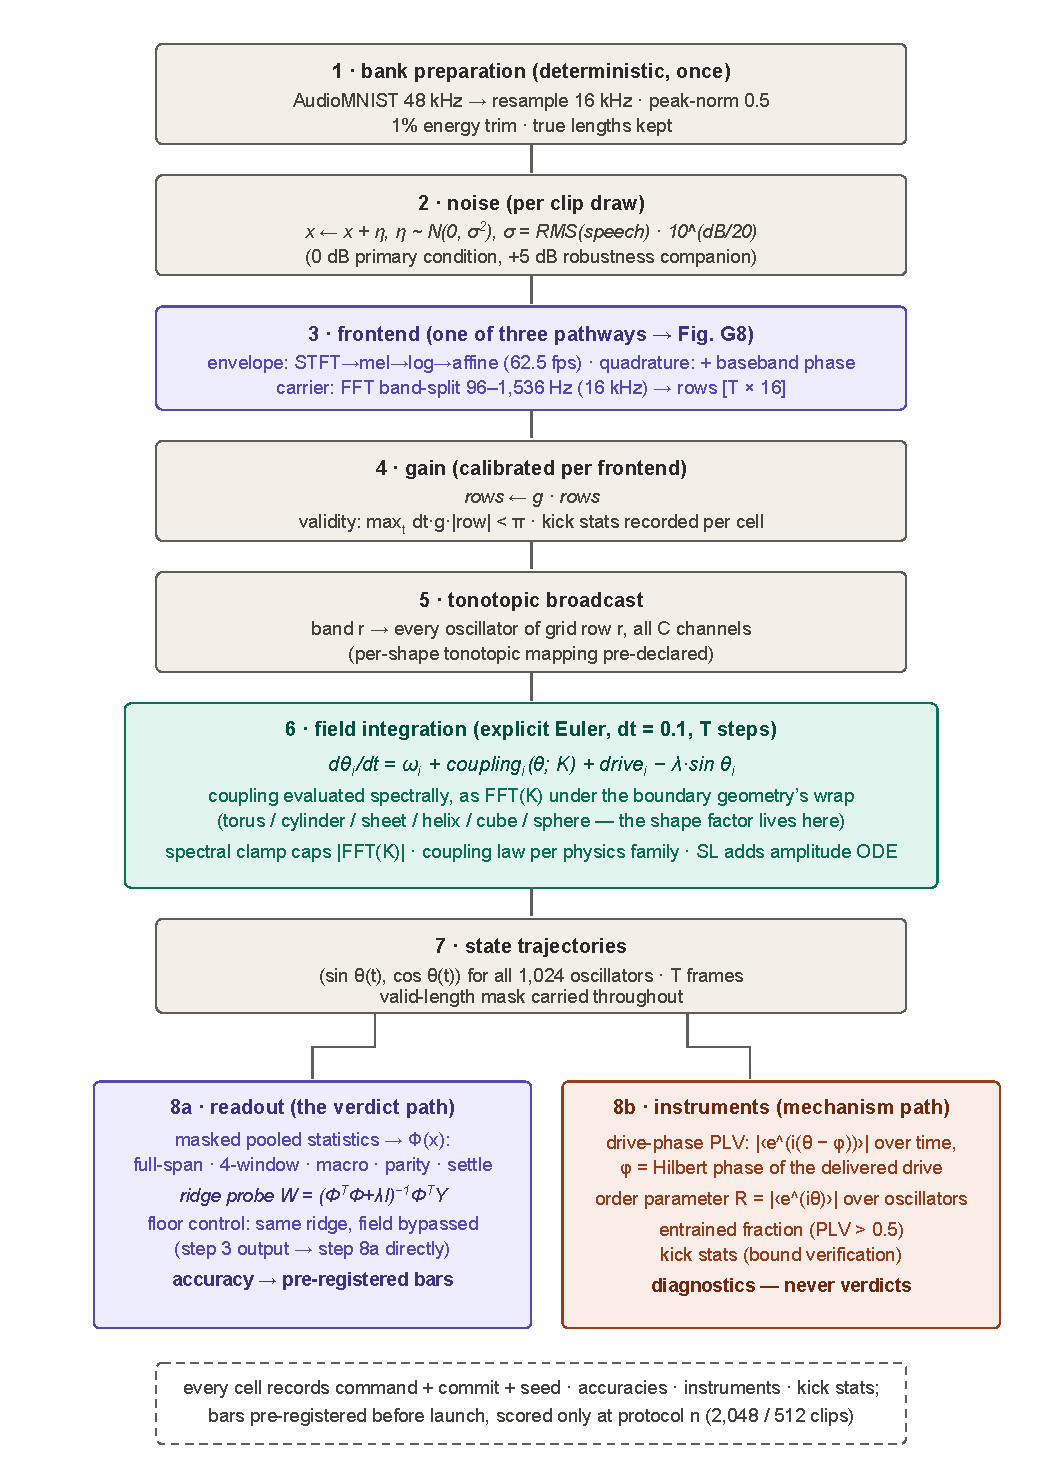
\includegraphics[keepaspectratio,alt={Order of operations, from audio to verdict. Every arm of the study passes through the same stages in the same order; only the boxed stage differs between an oscillator arm and its floor.}]{resources/figures/g0-pipeline-order.pdf}}
\caption{Order of operations, from audio to verdict. Every arm of the
study passes through the same stages in the same order; only the boxed
stage differs between an oscillator arm and its floor.}
\end{figure}

\begin{figure}
\centering
\pandocbounded{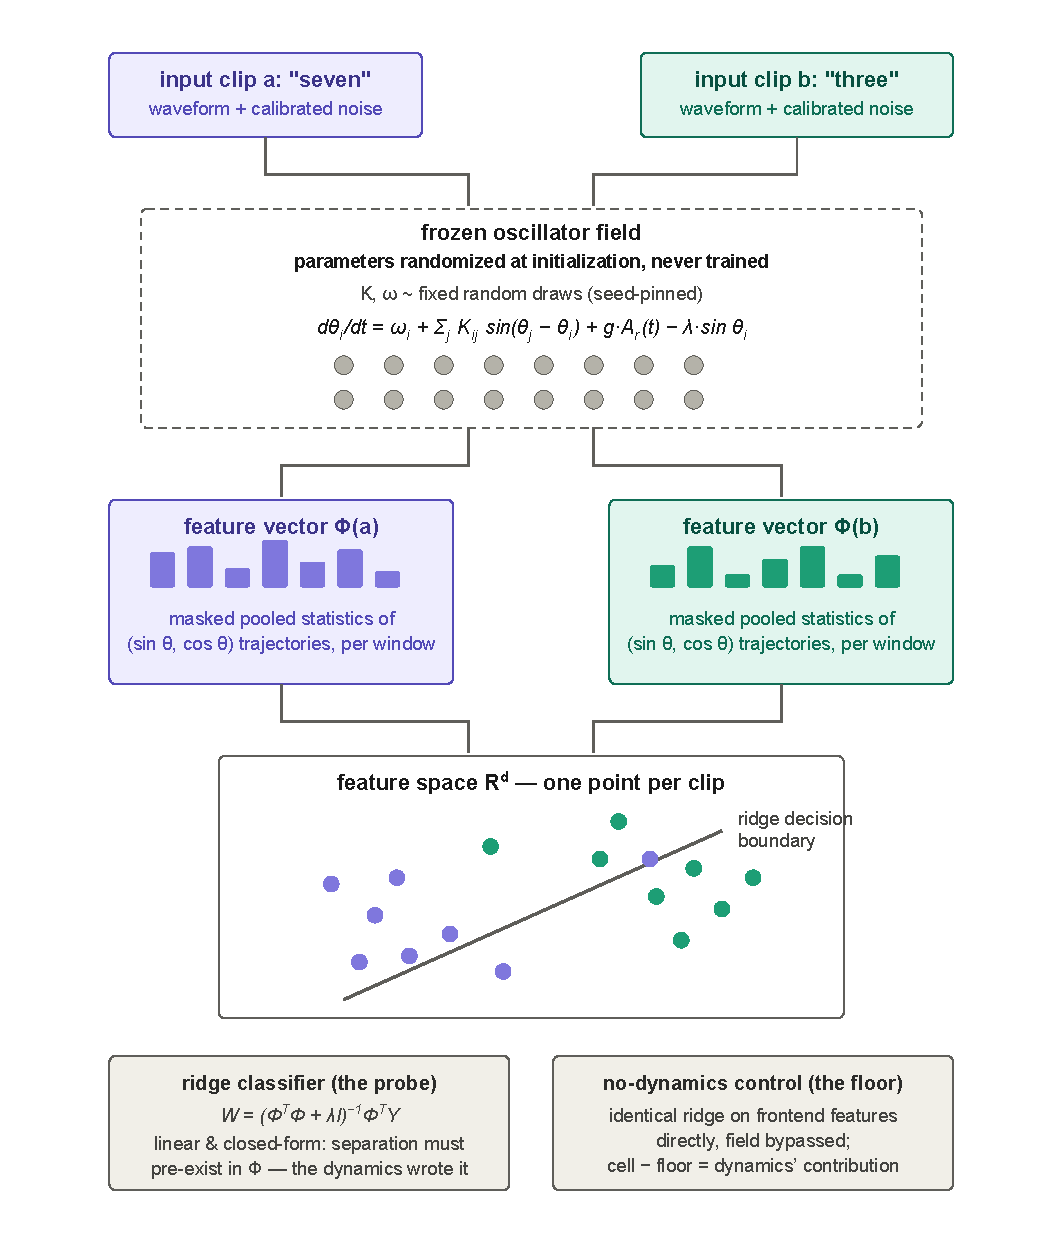
\includegraphics[keepaspectratio,alt={The linear-probe attribution protocol. The probe is deliberately the weakest available reader, so that any separation it finds must already exist in the features rather than being computed by the readout.}]{resources/figures/g7-probe-mechanism.pdf}}
\caption{The linear-probe attribution protocol. The probe is
deliberately the weakest available reader, so that any separation it
finds must already exist in the features rather than being computed by
the readout.}
\end{figure}

\section{Methods}\label{methods}

\subsection{Task and data}\label{task-and-data}

AudioMNIST \citep{becker2024}: 30,000 recordings, 60 speakers
\ensuremath{\times} 10 digits \ensuremath{\times} 50 repetitions at 48
kHz. Bank: repetitions 0--19 per speaker\ensuremath{\times}digit,
resampled to 16 kHz, peak-normalized to 0.5, energy-trimmed at 1\% of
peak, \ensuremath{\leq}1 s, true lengths stored; speaker-disjoint split
(speakers 1--48 train / 49--60 test; overlap verified zero). Median
digit 0.62 s = 38 hop frames. Training/evaluation sets are drawn from
the bank with replacement (repeated clips receive fresh noise draws);
the protocol size is 2,048 training / 512 test clips per run, and all
decision bars are scored only at this size.

\subsection{Primary frontend (mel
envelope)}\label{primary-frontend-mel-envelope}

512-sample/256-hop Hann STFT \ensuremath{\to} 16 mel bands
\ensuremath{\to} log \ensuremath{\to} fixed affine (v+10)/10 clamped at
0 \ensuremath{\to} rows {[}T\ensuremath{\times}16{]} at 62.5 fps. Zero
trainable parameters and no per-utterance statistics (streaming
honesty); deliberately lightweight so bookend projections cannot
dominate attribution. Constants calibrated on the digit bank (1,024
clips, valid frames only): raw log-mel first percentile
\ensuremath{-}7.74 (the \ensuremath{-}10 offset sits below it);
post-affine mean 0.84 / p95 1.52 / max 1.80; clamped fraction 0.02\%.
Disclosures: 50\% window overlap \ensuremath{\Rightarrow} adjacent-frame
correlation, identical for every arm; no overlap across clips. A
lens-cost control runs one conventional baseline at 40 mel bands so the
16-band bottleneck's cost is a measured number in anchor comparisons.

\subsection{The transduction ladder (drive
pathways)}\label{the-transduction-ladder-drive-pathways}

Three pathways are chosen so each adds exactly one kind of information
or mechanism over the last, making result differences attributable to
that addition:

\begin{itemize}
\tightlist
\item
  \textbf{Envelope (mel)}. Loudness only: the frontend above; drive
  \ensuremath{\dot{\theta}_{i}} +=
  g\ensuremath{\cdot}A\ensuremath{_{r}}(t), additive and
  state-independent. The base rung: literature-standard representation,
  comparable to the baselines and anchors.
\item
  \textbf{Quadrature}. Adds reference-relative phase at the same rate
  and bands: the per-band analytic signal demodulated at band center
  yields a baseband phase \ensuremath{\varphi_{r}}(t)
  (\ensuremath{\pm}31 Hz by the hop Nyquist, never raw carrier cycles);
  drive \ensuremath{\dot{\theta}_{i}} +=
  g\ensuremath{\cdot}A\ensuremath{_{r}\cdot}sin(\ensuremath{\varphi_{r}}
  \ensuremath{-} \ensuremath{\theta_{i}}), the canonical Adler injection
  form \citep{adler1946}.
\item
  \textbf{Carrier (direct)}. Removes the transcoder: a full-clip FFT
  band-split (16 bands, 96--1,536 Hz) delivers the band waveforms
  themselves at 16 kHz; drive \ensuremath{\dot{\theta}_{i}} +=
  g\ensuremath{\cdot}x\ensuremath{_{r}}(t), additive and oscillatory, so
  genuine injection locking becomes possible. Its band limit trades the
  \textgreater1.5 kHz envelope information the mel path keeps for
  in-band carrier phase, priced by computing every floor on the carrier
  representation itself (§5.3).
\end{itemize}

\begin{figure}
\centering
\pandocbounded{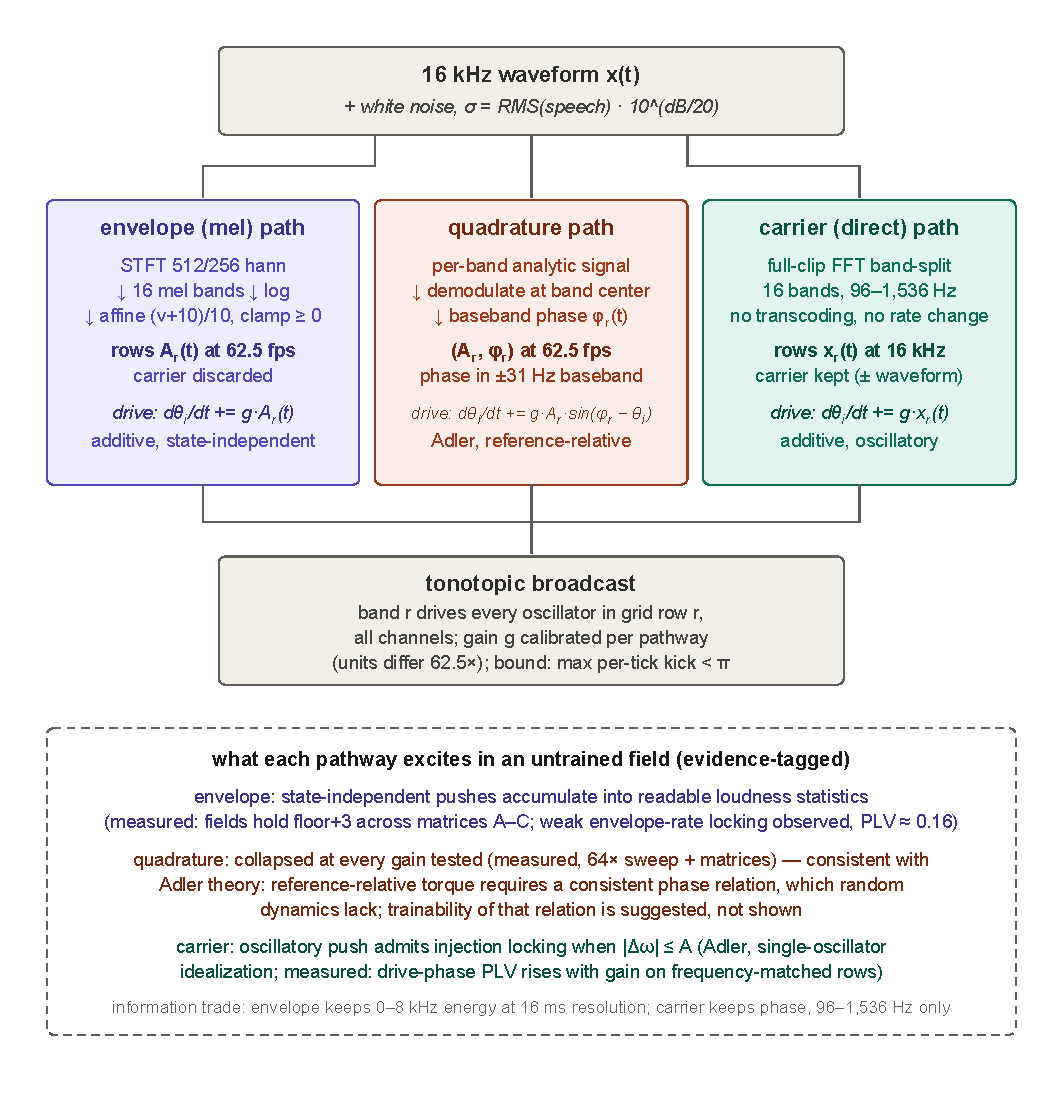
\includegraphics[keepaspectratio,alt={The three drive pathways. Each rung adds exactly one kind of information or mechanism over the one below it, so a difference in result is attributable to that addition.}]{resources/figures/g8-drive-pathways.pdf}}
\caption{The three drive pathways. Each rung adds exactly one kind of
information or mechanism over the one below it, so a difference in
result is attributable to that addition.}
\end{figure}

Evidence notes carried with the ladder: envelope pushes accumulate into
readable loudness statistics (measured throughout §5.2), and the
measured weak envelope-rate locking (drive-phase PLV
\ensuremath{\approx} 0.16 at the calibrated operating point, decaying
with gain) \emph{suggests additive drive} can weakly phase-lock through
the pinning nonlinearity, the Shapiro-step mechanism
\citep{pikovsky2001}, while carrying no claim that it must. Quadrature
collapsed at every gain tested (§5.2, §6), consistent with Adler theory;
trainability of the required phase relation is suggested, not shown.
Carrier drive admits injection locking when
\textbar{}\ensuremath{\Delta\omega}\textbar{} \ensuremath{\leq} A
(single-oscillator idealization; measured in §5.3).

\subsection{Noise protocol}\label{noise-protocol}

Added white noise with \ensuremath{\sigma} = RMS(speech)
\ensuremath{\cdot} 10\^{}(dB/20), drawn i.i.d. per sample over the full
padded window; 0 dB means noise at speech-equal power (not clean audio),
\ensuremath{-}10 dB means 0.32\ensuremath{\times}, +5 dB means
1.78\ensuremath{\times}. Why noise at all: the unmodified samples
saturate the models under test (untrained arms reach 0.939 already at
\ensuremath{-}10 dB, brushing our 0.95 kill line), and a near-ceiling
task cannot discriminate design points. Calibration: a
\{\ensuremath{-}10\ldots+10 dB\} grid over four untrained arms; pick the
level whose strongest untrained arm lands in {[}0.70, 0.90{]}.
Conditions of record: \textbf{0 dB primary, +5 dB as the harsher-noise
robustness companion}, both fully run under both baseline protocols,
both reported. Listenable examples (the same clip at every level, one
seeded noise draw rescaled per level) ship with the paper, regenerable
by a committed script.

\subsection{Drive scale, gain, and the integrator-validity
bound}\label{drive-scale-gain-and-the-integrator-validity-bound}

The gain dial multiplies frontend-relative units, so cross-frontend gain
equality is meaningless: measured row scales at 0 dB are mel-affine RMS
1.32 versus carrier RMS 0.021, a 62.5\ensuremath{\times} units gap. Each
frontend therefore runs at its own gate-calibrated gain, with effective
drive (g \ensuremath{\times} row RMS) reported at every operating point.
Gains of record: mel g = 1.0 (the calibrated units unamplified; its gate
read flat \ensuremath{\pm}0.6 across \{0.5, 1, 2\}); carrier g = 32 by
its own gate. Every sweep obeys an integrator-validity bound: a point is
valid iff every per-tick drive phase increment stays below
\ensuremath{\pi} (max-criterion; standard explicit-integrator discipline
\citep{hairer1993}), with rms increment \ensuremath{\leq} 0.5 rad as an
accuracy annotation. Measured bounds: carrier valid to g
\ensuremath{\approx} 75, mel to g \ensuremath{\approx} 17 at dt = 0.1.
Per-run increment statistics are recorded by instrumentation in every
run. Higher physical drive, when a question needs it, is reached by
increasing substeps, never by gain past the bound. Prior art for the
response shape: input scaling is a canonical reservoir hyperparameter
with an interior optimum \citep{lukosevicius2012}.

\subsection{Instrumentation (mechanism, never
verdicts)}\label{instrumentation-mechanism-never-verdicts}

Drive-phase PLV per band: each oscillator's phase is compared against
the analytic (Hilbert) phase of its own row's \emph{delivered drive};
entrained fraction is the share above a 0.5 lock threshold. Rationale:
natural stimuli have no single analytic stimulus phase, but the
delivered drive is fully known, and locking to it is the physically
meaningful question and is well-defined for every stimulus class here.
On pure tones, where a stimulus phase is analytic, the drive-phase
reader agrees with the stimulus-phase reader (committed test). The
global order parameter \(R = |\langle e^{i\theta}\rangle|\) (no
reference; the field against itself) and the per-tick drive-increment
statistics complete the instrument set. Instruments are diagnostics;
verdicts come only from the pre-registered accuracy bars.

\subsection{Evidential standard}\label{evidential-standard}

\textbf{Scope and evidence.} Speech recognition from frozen oscillator
fields. Every number reported here comes from a pre-registered,
protocol-complete run; decision criteria were written before each run
and verdicts scored per the criteria as written. All code, per-run
results, and audio and figure assets accompany the paper (§9).

Pre-registration with bars written before launch; frozen controls
through identical scaffolding; replication (screens at one seed; claims
need three seeds plus same-seed replicates, seeds matched across arms);
cross-run and same-seed determinism checks (bit-identical replication
verified); best-validation selection under one rule for all arms. Every
run records command + commit + seed, accuracies per feature family,
instruments, and drive-increment statistics.

\section{Results}\label{results}

Throughout: ``windowed'' is the primary metric (the ridge on
per-quarter-window pooled statistics); floors are per-condition and
per-representation; chance is 0.100.

\subsection{Conventional references at exact parameter
parity}\label{conventional-references-at-exact-parameter-parity}

Five trained baselines (GRU, TCN, small CNN, tiny transformer, minimal
S4D-style SSM) at the matched \textasciitilde2k budget, identical
frontend, featurization, ridge, and selection protocol, under two
protocols: the \emph{frozen-probe} protocol (training against a fixed
random readout direction, the physics-symmetric objective used by field
arms) and the \emph{trained-head} protocol (a learned classifier head,
conventional practice), three seeds each, at both noise conditions.

Trained-head windowed means (per-seed tables in the supplementary
results):

{\def\LTcaptype{none} % do not increment counter
\begin{longtable}[]{@{}lll@{}}
\toprule\noalign{}
arm & +5 dB & 0 dB \\
\midrule\noalign{}
\endhead
\bottomrule\noalign{}
\endlastfoot
GRU & \textbf{0.737} & 0.772 \\
\cmidrule{1-3}CNN & 0.703 & 0.741 \\
\cmidrule{1-3}Transformer & 0.697 & \textbf{0.776} \\
\cmidrule{1-3}TCN & 0.693 & 0.767 \\
\cmidrule{1-3}S4D & 0.685 & 0.746 \\
\end{longtable}
}

Two findings frame everything downstream. First, \textbf{at the 2k
budget, trained conventional networks approximately equal a linear ridge
on band statistics}: at +5 dB only one trained run of thirty (GRU seed
2, 0.762) exceeds the windowed floor (0.750), and at 0 dB zero
trained-head runs clear the floor (0.805; closest 0.801). Second, a
scaffold finding: the frozen-probe objective is hostile to ReLU
feed-forward architectures (CNN/TCN collapse under it while training
fine conventionally at the same size), measured by a
scaffold-versus-size control with learned heads at the identical budget.
Both protocols are therefore reported for every conventional arm.
Literature anchors, with protocol caveats and never as head-to-head
claims: spintronic hardware reservoirs \textasciitilde99.6\% on TI-46
\citep{torrejon2017}; coRNN on AudioMNIST 78--91\% under different
frontends \citep{rusch2021}.

\subsection{The untrained matrix: a statics plateau, with design effects
bounded below
threshold}\label{the-untrained-matrix-a-statics-plateau-with-design-effects-bounded-below-threshold}

The full factorial (six physics \ensuremath{\times} six geometries
\ensuremath{\times} three \ensuremath{\omega} levels \ensuremath{\times}
two \ensuremath{\lambda} \ensuremath{\times} two clamp
\ensuremath{\times} two frontends) ran at three conditions: A (+5 dB,
g=2), B (0 dB, g=2), C (+5 dB, g=1): 600 supported runs each (documented
implementation scopes exclude SL \ensuremath{\times} non-torus and SL
\ensuremath{\times} quadrature), with the sakaguchi/harmonic2 columns
measured at their canonical nonzero parameters. Verdicts per the
pre-registered bars:

\textbf{The plateau.} Envelope-driven untrained fields hold
\ensuremath{\approx} floor+3 at every condition. Means (vs windowed
floors): A 0.774 (0.750), B 0.836 (0.805), C 0.783 (0.750); maxima
0.79--0.87, topping every trained conventional mean at the 2k budget
under both protocols at both noise levels, while never exceeding their
own representation's linear content by more than a few points. At this
scale, digit identity is statics-dominated, and everything reaches it.

\textbf{Geometry: little impact beyond the control, replicated.} Every
shape is compared against its torus twin, the run identical to it in
physics family, \ensuremath{\omega} structure, pinning, clamp, and
operating condition, differing only in the lattice wrap rule. Under
envelope drive each shape has 48 such twins per condition (four phase
families \ensuremath{\times} three \ensuremath{\omega}
\ensuremath{\times} two \ensuremath{\lambda} \ensuremath{\times} two
clamp; the amplitude cores are torus-only and so contribute none), and
144 pooled across the three conditions.

No shape came close to the pre-registered +3 threshold. Pooled over the
three conditions, the per-shape mean deltas run from \ensuremath{-}0.13
(sphere) to +0.39 (helix); helix, the best shape, is positive in 61\% of
its 144 twins. Read one condition at a time, the extremes widen only to
\ensuremath{-}0.63 (sphere, +5 dB g=1) and +0.58 (helix, +5 dB g=2),
still under a fifth of the threshold, and not consistent in sign across
conditions for any shape but helix. The quadrature pathway agrees
despite sitting near chance: \ensuremath{-}0.53 to +0.29 over the same
144 twins per shape. To our knowledge this is the first controlled
geometry comparison in an oscillator network; at this scale, the
measured effect of lattice shape is bounded well below our decision
threshold.

\textbf{Tonotopic design: no measured benefit over its randomized
control, replicated.} The pre-registered criterion required designed
\ensuremath{\omega} to exceed \emph{randomized} \ensuremath{\omega} (the
randomized-twin discipline of \citep{caranzano}) by +5. It was not met
on any read, at any scope.

Per physics family, pooled over the three conditions under envelope
drive (72 twins per phase family, 12 per amplitude family), designed
\ensuremath{-} random runs from +0.28 (kuramoto) down to
\ensuremath{-}1.21 (harmonic2), with no family reaching a tenth of the
bar, and harmonic2 and winfree negative in all three conditions. Pooling
families within a condition (104 twins), the envelope deltas are
\ensuremath{-}0.31, \ensuremath{-}0.42 and \ensuremath{-}0.56; on the
widest read available, all families and both drive pathways at one
condition (200 twins), they are \ensuremath{-}0.12, +0.52 and
\ensuremath{-}0.60. Under envelope drive the carrier is absent at hop
rate, so \ensuremath{\omega} structure can act only as a timescale
prior, and we measured no untrained benefit from it.

\textbf{Gain: near-dead, with one named interaction.} Full-matrix
C\ensuremath{-}A deltas: +0.9 mean (73\% positive), a small real tilt
toward g=1, with every factor summary below the \ensuremath{\pm}3
yardstick except one: \textbf{fixed-amplitude SL recovers +3.3 at g=1},
erasing its Matrix-A deficit. The physics-family spread is therefore
operating-point-conditioned (3.3 points at g=2 compressing to
\textasciitilde1.2 at g=1), and amplitude freedom reads as the absorber
of drive-scale mismatch: full SL was gain-insensitive; only the
amplitude-clamped variant moved.

\textbf{Coupling law barely matters untrained.} With genuinely distinct
physics (\ensuremath{\alpha} = \ensuremath{\pi}/4, \ensuremath{\beta} =
0.5), per-twin deviations from kuramoto are +0.1 to +0.9 points
(\ensuremath{\approx} half positive; 72 twins per family per condition):
sl 0.783 \textgreater{} kuramoto \ensuremath{\approx} sakaguchi
\ensuremath{\approx} harmonic2 (\ensuremath{\approx}0.776)
\textgreater{} winfree 0.773 \textgreater{} sl-fixedamp 0.750 at g=2.
Within phase cores, the coupling law is worth under a point untrained;
the amplitude channel is the only physics lever above one.

\textbf{Phase-referenced drive: collapsed at every gain.} Quadrature
runs sit at 0.24--0.33 absolute (chance 0.10), \ensuremath{-}0.53 below
their magnitude twins at 100\% of 288 twin pairs, and a diagnostic sweep
at g \ensuremath{\in} \{8, 32, 128\} plus the matrix's g
\ensuremath{\in} \{1, 2\} never recovers half the magnitude read
(non-monotone, \ensuremath{\leq}0.324 throughout). The identical
quadrature pathway trains healthily (+39.8\% loss drop in harness
verification). Section 6 gives the model analysis; the scoped claim is
that \textbf{phase-referenced input is trainable-but-not-reservoir}.

\textbf{Settle-versus-stream.} Every frozen run was read both ways: from
the driven streaming trajectory, and from a 32-frame drive-free
ring-down. Settle loses everywhere: \ensuremath{-}10 points mean, 0\%
positive across 600 runs. For untrained envelope-driven fields, the
driven trajectory carries the information.

\subsection{The transduction test: carrier drive does not rescue the
plateau}\label{the-transduction-test-carrier-drive-does-not-rescue-the-plateau}

If the mel transcoder were compressing a dynamical margin, driving the
field with the band-split waveform itself (the carrier pathway) should
restore it. We measured carrier floors first (0 dB: standard 0.533,
windowed 0.680; the \ensuremath{\approx}12-point gap to the mel floors
is the band-limit's measured cost), gate-calibrated the carrier gain
(g=32), and ran a 14-run diagonal (six physics \ensuremath{\times} torus
\ensuremath{\times} \{random, designed\} \ensuremath{\omega} + a helix
pair) at protocol size, with three pre-registered bars. All three came
back negative:

\begin{enumerate}
\def\labelenumi{\arabic{enumi}.}
\tightlist
\item
  \textbf{Transduction:} best run 0.701 = carrier floor +2.1 (bar: +5 to
  claim restoration; \ensuremath{\leq}+3 \ensuremath{\Rightarrow}
  statics-bound is frontend-invariant). Thirteen of fourteen runs sit at
  or below the carrier floor. The statics-bound picture holds under both
  transduction modes.
\item
  \textbf{Tonotopic design under carrier drive:} designed \ensuremath{-}
  random averaged \textbf{\ensuremath{-}2.0} across the diagonal's seven
  designed/random twins, and the same to one decimal over the six torus
  families alone (criterion: +5). The no-benefit finding extends to the
  drive form the design was meant for. The instrument sharpens the
  point: designed rows demonstrably lock to their carriers (drive-phase
  PLV 0.17 vs 0.03 for random rows, 5--6\ensuremath{\times}) \emph{and
  score lower}. Our results showed that entrainment occurs; it did not
  improve accuracy on this task at this scale.
\item
  \textbf{Helix octave-per-turn:} +1.0 / \ensuremath{-}1.0 vs torus
  (criterion: +3). The geometry finding extends unchanged to carrier
  drive.
\end{enumerate}

\textbf{Drive-pathway mechanism, summarized from the measurements
above.} Our results showed the envelope representation's floor at 0.805
against the carrier's 0.680: the representation itself carries
\textasciitilde12.5 points more linearly readable content, because the
band-split path discards all envelope information above 1.5 kHz, while
the field added a similar small margin above each floor. The instruments
showed weak envelope-rate locking on the winning pathway (drive-phase
PLV \ensuremath{\approx} 0.16) and strong carrier locking on the losing
designed rows (5--6\ensuremath{\times} the random arm's PLV). Together
these measurements support a representation-content account of the
pathway ordering and count against a resonance-matching account: the
pathway with the least locking won, and the pathway with the most
locking gained nothing from it. We therefore attribute the envelope
path's advantage to what its representation carries, not to how its
drive engages the physics; we hypothesize that locking becomes valuable
only when the task requires the temporal structure it encodes, a
hypothesis §5.7 begins to test and that direct per-band transduction
instrumentation would settle.

The gain-response curves behind the operating points were re-verified at
three seeds with the drive-phase reader and the increment instrument
(quotable table in supplementary): designed-\ensuremath{\omega} holds a
seed-robust +3--4 point edge over random at gate size in the mid-gain
band, an edge that vanishes at protocol size, which is why the scored
Caranzano verdict is negative. Locking is a mechanism; the probe scores
outcomes.

\subsection{Readout sufficiency: the linear probe,
tested}\label{readout-sufficiency-the-linear-probe-tested}

The weakest-reader design choice is a measured control, not an
assumption. On one scored-condition run and its floor twin, an MLP head
(2\ensuremath{\times}128) and a small window-token transformer ran on
the \emph{identical} features, identical splits and selection, three
head seeds, across training sizes 512\ensuremath{\to}16,384
(with-replacement caveat: the pool holds 9,600 unique clips; the largest
size is an augmentation regime and labeled as such).

At protocol size (2,048): the transformer reads +2.6 over ridge on run
features (all three seeds above) while reading \ensuremath{-}10 on the
floor twin: a real, seed-robust, run-side-only nonlinear margin, and the
honest caveat to linear-completeness. It is a small-data phenomenon: by
4,096 the ridge saturates the run read (0.871), by 16,384 the ridge
leads everything (0.881), and the floor's own nonlinear readers close
most of the remaining gap (floor MLP +2.3 over floor ridge at 8,192;
generic band-statistic nonlinearity, not field structure). Across the
whole curve, the field's best-reader edge over its floor's best reader
is stable at +1.7 to +2.9 points. Overfitting is reported, not assumed:
every nonlinear head shows train--test gaps of +0.09 to +0.20, and the
floor MLP memorizes its training set outright. All heads carry more
parameters than the entire oscillator field.

\subsection{Sensitivity of the canonical physics
values}\label{sensitivity-of-the-canonical-physics-values}

\textbf{harmonic2 \ensuremath{\beta}:} deviations from kuramoto are
identical (\ensuremath{-}0.98) at \ensuremath{\beta} \ensuremath{\in}
\{0.25, 0.5, 1.0\}, insensitive across the literature range
\citep{hansel1993, daido1992} (verified to be a genuine accuracy
plateau, not a plumbing artifact: the trajectories differ substantially
between \ensuremath{\beta} values). \ensuremath{\beta} \textgreater{} 1
is excluded by design: the second-harmonic weight multiplies its term
unnormalized, confounding coupling shape with total strength; a future
extension would use normalized mixing (1,
\ensuremath{\beta})/(1+\ensuremath{\beta}).

\textbf{sakaguchi \ensuremath{\alpha}:} the five-point response
\{\ensuremath{\pi}/8, \ensuremath{\pi}/4, 3\ensuremath{\pi}/8, 1.39,
\ensuremath{\pi}/2\} traces a non-monotone curve: +0.2 /
\ensuremath{-}2.7 / \ensuremath{-}3.9 / \ensuremath{-}0.4 / +1.2 versus
kuramoto (each point \ensuremath{\leq}1.7\ensuremath{\sigma}
individually; the trough \ensuremath{\approx}2.4\ensuremath{\sigma}). A
registered mechanistic prediction, that the deviation tracks frustration
energy \ensuremath{\propto} sin 2\ensuremath{\alpha} and is therefore
symmetric about \ensuremath{\pi}/4, was \textbf{refuted} by the
3\ensuremath{\pi}/8 point. The instruments show the lag desynchronizing
the field monotonically (R 0.095 \ensuremath{\to} 0.066 across the
range; textbook Sakaguchi behavior) while envelope locking stays flat,
so readability does not track coherence, and the least synchronized
field (\ensuremath{\alpha} = \ensuremath{\pi}/2, the zero-attraction
boundary) reads best, slightly above kuramoto. \ensuremath{\alpha}
therefore enters the record as a measured factor level with its response
curve (\ensuremath{\pi}/4 = mid-range lag; 1.39 = \ensuremath{\pi}/2
\ensuremath{-} 0.18, the canonical chimera value \citep{abrams2004};
\ensuremath{\pi}/2 = the boundary), not an assumed constant.
Matrix-wide, the family deviation at \ensuremath{\alpha} =
\ensuremath{\pi}/4 is +0.1--0.2 (§5.2): the crown-configuration trough
did not generalize.

\subsection{Coherence and readability: an inverted-U,
suggested}\label{coherence-and-readability-an-inverted-u-suggested}

A registered scatter over the corrected protocol-size matrices (936
envelope runs: 312 at each of the three conditions) tested whether
readability anti-correlates with global coherence. The anti-correlation
bar (Spearman \ensuremath{\rho} \ensuremath{\leq} \ensuremath{-}0.3 in
\ensuremath{\geq}2 of 3 conditions) came back 0/3: the across-run trend
at low coherence is mildly \emph{positive} and consistent
(\ensuremath{\rho} = +0.256, +0.254, +0.227; winfree +0.51 to +0.62 per
condition). Meanwhile every high-coherence state we measured reads worse
than its less-coherent twin: the reference-slaved quadrature regime; the
most coherent carrier run (R 0.65) losing to its incoherent twin (R
0.32); the \ensuremath{\alpha}-curve's locked extremes. The recorded
suggestion, which is a suggestion and not a mechanism, is
\textbf{non-monotone: mild coherence helps, locking hurts} (an
inverted-U in R). Across-run correlations are confounded (R co-varies
with pinning, clamp, and family), so the named discriminating experiment
is a causal within-family R-response curve, driving R from
\textasciitilde0.05 to \textasciitilde0.6 with everything else fixed.
This reading is consistent with the over-synchronization concerns raised
independently in the trained-oscillator literature
\citep{unconv-ai2026, nunley2026}.

\begin{figure}
\centering
\pandocbounded{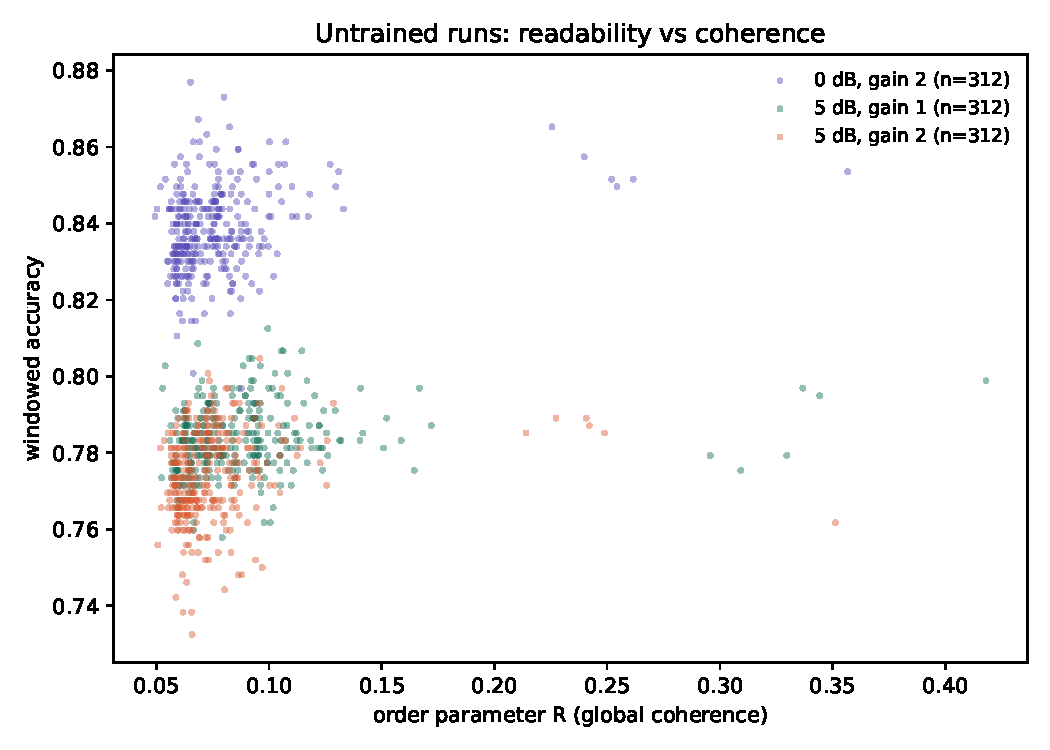
\includegraphics[keepaspectratio,alt={Readability against coherence across the swept conditions. The relation is not monotone: mild coherence accompanies the best reads, and the most strongly locked fields read worse than their less coherent twins.}]{resources/figures/g9-readability-vs-coherence.pdf}}
\caption{Readability against coherence across the swept conditions. The
relation is not monotone: mild coherence accompanies the best reads, and
the most strongly locked fields read worse than their less coherent
twins.}
\end{figure}

\subsection{The task axis: untrained state carries temporal order
near-perfectly}\label{the-task-axis-untrained-state-carries-temporal-order-near-perfectly}

Every task above is statics-dominated, so the field's dynamics are
barely interrogated. We therefore built a task that statics provably
cannot answer: classify two-digit sequences whose unordered content is
identical (digit a then b, versus b then a; independent recordings
joined by a 100 ms gap; a 272 ms silent leader absorbs the featurization
warmup so the readout window is order-symmetric by design). The primary
read is the full-span pooled protocol, which is order-free by
construction: any permutation-invariant statistic of the frame multiset
is identical for both classes regardless of its richness: the defense is
mathematical, not empirical, though the empirical check agrees (matched
floors 0.465--0.518 across all five pairs; chance 0.500; the
\textbar{}\ensuremath{\Delta}\textbar{} feature's single-junction
sensitivity is the stated exception and is measurably negligible). Any
accuracy above chance through this readout must come from state that
persists across time.

Results (five digit pairs, three seeds, protocol size; full-span
accuracy):

{\def\LTcaptype{none} % do not increment counter
\begin{longtable}[]{@{}
  >{\raggedright\arraybackslash}p{(\linewidth - 8\tabcolsep) * \real{0.2000}}
  >{\raggedright\arraybackslash}p{(\linewidth - 8\tabcolsep) * \real{0.2000}}
  >{\raggedright\arraybackslash}p{(\linewidth - 8\tabcolsep) * \real{0.2000}}
  >{\raggedright\arraybackslash}p{(\linewidth - 8\tabcolsep) * \real{0.2000}}
  >{\raggedright\arraybackslash}p{(\linewidth - 8\tabcolsep) * \real{0.2000}}@{}}
\toprule\noalign{}
\begin{minipage}[b]{\linewidth}\raggedright
pair
\end{minipage} & \begin{minipage}[b]{\linewidth}\raggedright
matched floor
\end{minipage} & \begin{minipage}[b]{\linewidth}\raggedright
kuramoto (frozen)
\end{minipage} & \begin{minipage}[b]{\linewidth}\raggedright
SL (frozen)
\end{minipage} & \begin{minipage}[b]{\linewidth}\raggedright
GRU (trained)
\end{minipage} \\
\midrule\noalign{}
\endhead
\bottomrule\noalign{}
\endlastfoot
3,7 & 0.486 & 0.970 \ensuremath{\pm}0.003 & 0.990 \ensuremath{\pm}0.004
& 0.977 \ensuremath{\pm}0.015 \\
\cmidrule{1-5}1,8 & 0.496 & 0.997 \ensuremath{\pm}0.003 & \textbf{1.000
\ensuremath{\pm}0.000} & 0.995 \ensuremath{\pm}0.001 \\
\cmidrule{1-5}2,5 & 0.490 & 0.997 \ensuremath{\pm}0.002 & 0.996
\ensuremath{\pm}0.004 & 0.992 \ensuremath{\pm}0.005 \\
\cmidrule{1-5}4,9 & 0.518 & 0.988 \ensuremath{\pm}0.005 & 0.995
\ensuremath{\pm}0.001 & 0.990 \ensuremath{\pm}0.004 \\
\cmidrule{1-5}0,6 & 0.465 & 0.988 \ensuremath{\pm}0.003 & 0.996
\ensuremath{\pm}0.002 & 0.995 \ensuremath{\pm}0.003 \\
\end{longtable}
}

(\ensuremath{\pm} = half-range over three seeds; audio examples of the
stimuli, both orders of two pairs at the experimental condition, ship
with the paper in \texttt{resources/audio/order/}, regenerable by
committed script.)

The pre-registered bar (\ensuremath{\geq}0.60 on \ensuremath{\geq}3 of 5
valid pairs) passes 5/5 with \textasciitilde40 points to spare:
\textbf{untrained oscillator state reads temporal order at 0.97--1.00
through readouts that are blind to it without the dynamics.} Frozen
Stuart--Landau is the best arm everywhere (amplitude as memory; one
perfect score), and the frozen fields match the trained GRU, a
comparison scoped strictly to the shared order-free readout protocol (a
recurrent network with a sequence head would answer this task trivially;
the point is that under identical readout constraints, training the
recurrence added nothing beyond what the frozen physics provides).

A severed-coupling control (spectral cap \ensuremath{\to} 0, same runs)
attributes the mechanism: uncoupled oscillators alone read 0.947--0.980,
with coupling adding +1.7--2.3, closely matching the coupling term's
measured contribution on the statics task. \textbf{The order memory is
predominantly per-oscillator phase integration}: each oscillator's phase
is an integral of its own drive history, with collective dynamics
contributing a small consistent margin. Scope notes: this is synthetic
sequencing of natural units (no co-articulation), one gap length, near
ceiling, a single demonstration with a registered hardness ladder
(longer sequences, variable gaps, memory-horizon curves), not a
characterized capability. It is also consistent with the settle result
(§5.2): the memory lives in the \emph{driven} evolution of the state,
not in autonomous ring-down persistence.

\section{The phase-referenced collapse: model and
mechanism}\label{the-phase-referenced-collapse-model-and-mechanism}

The magnitude push is oscillator-state-independent; the Adler torque
g\ensuremath{\cdot}A\ensuremath{_{r}\cdot}sin(\ensuremath{\varphi_{r}}
\ensuremath{-} \ensuremath{\theta_{i}}) depends on each oscillator's
phase relative to a shared reference. The Adler equation
\ensuremath{\dot{\theta}} = \ensuremath{\Delta\omega} +
A\ensuremath{\cdot}sin(\ensuremath{\varphi-\theta}) locks iff
\textbar{}\ensuremath{\Delta\omega}\_eff\textbar{} \ensuremath{\leq} A
\citep{adler1946}; locking is the only mechanism by which a
reference-relative torque produces a persistent readable phase relation.

The untrained field sits outside the readable regime at every gain, for
two reasons that meet in the middle. At low gain, the baseband reference
rotates at up to \ensuremath{\pm\pi} rad/frame (the \ensuremath{\pm}31
Hz Nyquist edge) while intrinsic rates are \textasciitilde0.1 rad/frame
and per-frame torque \ensuremath{\lesssim}0.2 rad: far outside the
locking range, sin(\ensuremath{\varphi-\theta}) time-averages toward
zero, and residual torques across a population with random initial
phases and dispersed \ensuremath{\omega} are mutually incoherent. At
high gain, the torque dominates any detuning and the population is
dragged onto the shared reference, \ensuremath{\theta_{i}}
\ensuremath{\to} \ensuremath{\varphi_{r}}(t): a reference-slaved state
is nearly input-invariant in the informative dimensions: within a row
all oscillators carry the same \ensuremath{\varphi_{r}}, and the
amplitude pattern A\ensuremath{_{r}}(t), which carries most digit
identity (the magnitude path's 0.77+ demonstrates it), is projected out
of the phase state. The measured non-monotone middle (0.168/0.275/0.314
at g = 8/32/128) is consistent with the crossover between the two
failure regimes. This account is labeled consistent-with-data; the
per-gain drive-phase instrumentation that would test it directly is left
to future work.

What training changes is neither the drive nor the phases but the
coupling kernel: reshaping the field's autonomous dynamics until the
population maintains a consistent phase relation to the reference, at
which point reference-relative torques sum constructively, the identical
pathway trains healthily. Hence the scoped claim:
\textbf{phase-referenced input is trainable-but-not-reservoir}: it
requires co-organization with the reference, which trained dynamics can
supply and random dynamics cannot. Because of this phenomenon, the
carrier pathway removes the transcoder and drives the field with the
band-filtered waveform itself: an additive oscillatory drive engages
entrainment, creating phase organization through the locking dynamics
with no pre-organization required, turning the untrained-phase question
into one about locking range rather than co-organization. Section 5.3
reports the outcome: locking occurs, and the plateau stands.

\section{Discussion}\label{discussion}

\textbf{The hypothesis, scored.} As tested, at \textasciitilde2k
parameters, on spoken digits, under three drive forms and three
conditions, the reservoir premise splits along the task axis. On
statics-dominated recognition, it survives only in a bounded form:
untrained fields carry digit information consistently above every
trained conventional baseline at the same budget, yet only +2--3 points
above their own representation's linear content, and that margin was
indifferent to every design axis we varied but one: geometry and
tonotopic design each showed little impact beyond their controls (the
latter even with measured locking), the coupling law was worth under a
point, and gain was nearly inert; the exception is the drive pathway,
where phase-referenced input was unreadable rather than merely worse. On
the order task, the one task whose answer requires memory, the premise
holds emphatically: near-ceiling accuracy over chance-blind floors,
carried predominantly by per-oscillator integration. The synthesis:
\textbf{the input representation determines what the field can encode
(measured by floors, not by resonance-matching); the task determines
whether the dynamics are interrogated at all; the readout determines how
much of the whole stack is harvested; and the field's untrained design,
whether shape, frequency structure or coupling law, determines almost
nothing.} The strong version of the design premise is refuted at this
scale by the bars as written; the state-memory premise is confirmed. The
amplitude channel is the one design element that mattered on both axes
(family lead on statics; best arm on order), and since
\ensuremath{\alpha}/\ensuremath{\beta} are precisely the parameters
training can adjust, amplitude trainability is the sharpest hypothesis a
trained-dynamics study should test next.

\textbf{What bounds the conclusion.} Four limitations, each with its
measured control or named test: readout capacity (controlled in §5.4,
near-complete, with a quantified small-data exception); readout data
size (measured to the bank's ceiling; an expanded bank is the named next
test); field size (2k parameters is one point on the size axis, and the
size-scaling curve is unmeasured here); and frontend conditioning (two
of three pathways here are lossy in different ways, so transduction
itself wants direct instrumentation). The statics-dominance of digit
identity is itself a scope condition: tasks with heavier temporal
structure may separate dynamics from statics where digits cannot.

\textbf{What the no-effect findings are worth.} The geometry result
answers an open question no controlled experiment had touched; the
design results (tonotopy, coupling law) bound how much of the oscillator
revival's promise can come for free; the phase-collapse analysis
converts a failed factor into a mechanism with a testable training-side
prediction; and the coherence--readability inverted-U, if it survives
its causal test, connects the untrained record to the
over-synchronization failure mode reported in trained oscillator
systems. The evaluation frame, comprising floors, parity, drive-unit
calibration with a validity bound, drive-phase instrumentation and
pre-registered bars, is reusable as-is for trained-dynamics studies, and
ships with this paper for exactly that purpose.

\section{Related work}\label{related-work}

Hardware oscillator reservoirs establish the premise's strongest
published support \citep{torrejon2017}; reservoir computing supplies the
frame and its cautions
\citep{jaeger2001, maass2002, lukosevicius2012, tanaka2019}.
Oscillator-inspired trained networks (coRNN \citep{rusch2021}; Neural
Wave Machines \citep{keller2023}; WONN \citep{dai2026}; AKOrN
\citep{miyato2025}) and Kuramoto-based generation \citep{unconv-ai2026}
motivate the frozen-versus-trained distinction this paper measures from
the frozen side. Synchronization theory supplies the analytical spine
\citep{winfree1967, kuramoto1975, sakaguchi1986, adler1946, pikovsky2001, strogatz2000};
chimera states {[}Kuramoto \& Battogtokh 2002; Abrams \& Strogatz
2004{]} ground the partial-coherence readings. The randomized-twin
discipline for designed structure follows \citep{caranzano}; frequency-
learning front-ends \citep{lostanlen, zeghidour} are the trained
counterpoint to our fixed tonotopy. The closest body of work to this
paper's premise is the neuro-oscillatory speech literature reviewed by
\citep{dogonasheva2026}, whose three model families
\citep{assaneo2020, doelling2023, pittman-polletta2021} all obtain their
rate flexibility from adaptation of some parameter, and none of which is
evaluated against a parameter-matched conventional baseline on a
recognition task. To our knowledge, no prior work varies
oscillator-network lattice topology under controls, runs a
pre-registered factorial of coupling laws untrained, or instruments
drive-phase locking against delivered drive in a speech setting.

\section{Reproducibility}\label{reproducibility}

Everything the paper rests on is published alongside it. The record
holds 1,940 runs: the 1,800-run two-pathway factorial, the 14-run
carrier diagonal, and 126 gates, controls, sweeps, and conventional
references.

{\def\LTcaptype{none} % do not increment counter
\begin{longtable}[]{@{}
  >{\raggedright\arraybackslash}p{(\linewidth - 2\tabcolsep) * \real{0.5000}}
  >{\raggedright\arraybackslash}p{(\linewidth - 2\tabcolsep) * \real{0.5000}}@{}}
\toprule\noalign{}
\begin{minipage}[b]{\linewidth}\raggedright
what
\end{minipage} & \begin{minipage}[b]{\linewidth}\raggedright
where
\end{minipage} \\
\midrule\noalign{}
\endhead
\bottomrule\noalign{}
\endlastfoot
experiment harness (field cores, the nine geometries, frontends, probes,
instruments, baselines) & \texttt{harness/} \\
\cmidrule{1-2}the sweep driver and the launch, scoring, figure, and
audio scripts & \texttt{harness/sweep.py}, \texttt{scripts/} \\
\cmidrule{1-2}harness test suite (contracts for every mechanism the
paper claims) & \texttt{tests/} \\
\cmidrule{1-2}the complete record: 1,940 runs, grouped one file per
drive variant and coupling law, each carrying its full configuration and
every metric & \texttt{results/} \\
\cmidrule{1-2}authored figures and the generated coherence scatter &
\texttt{resources/figures/} \\
\cmidrule{1-2}noise-calibration and order-task audio examples &
\texttt{resources/audio/} \\
\end{longtable}
}

Every run records its full configuration and seed in its own
\texttt{results.json}; all matrices, gates, floors, and controls are
regenerable from the committed scripts. Same-seed replication is
bit-identical (verified cross-run and cross-run); cross-seed spreads are
reported wherever claims rest on them. Both registered predictions that
their own tests refuted (§5.5, §5.6) are reported in full above rather
than dropped.

\bibliography{references}
\end{document}
